\documentclass[a4paper,12pt,twoside,english]{article}
%% Language and font encodings
\usepackage[english]{babel}
\usepackage[utf8x]{inputenc}
\usepackage[T1]{fontenc}
\usepackage[affil-sl]{authblk} %for authors affiliations

%% Sets page size and margins
\usepackage[a4paper,top=3cm,bottom=2cm,left=3cm,right=3cm,marginparwidth=1.75cm]{geometry}

%% Useful  math packages
\usepackage{amssymb,amsmath,amsthm}
%% Useful  plot packages
\usepackage{float}
\usepackage{subfigure,color,colordvi,graphicx,xcolor}
%% Useful  table and list packages
\usepackage{array}
\usepackage{enumerate}
%% Create box
\usepackage[listings]{tcolorbox}
\newenvironment{myintro}[1]{%
	\tcolorbox[savedelimiter=mybox,
		savelowerto=\jobname_bspsave2.tex,
		lowerbox=ignored,
		colback=white,colframe=black,fonttitle=\bfseries,title=#1]}%
{\endtcolorbox}
%% Todo notes
\usepackage{todonotes}


\begin{document}
\title{Assignment 1}

%\author{Matteo Giacomini, Ruben Sevilla and Antonio Huerta}
\author[1]{Shushu Qin}
% \author[2]{Ruben Sevilla}
\affil[1]{{\small Laboratori de C\`alcul Num\`eric (LaC\`aN), ETS de Ingenieros de Caminos, Canales y Puertos, Universitat Polit\`ecnica de Catalunya, Barcelona, Spain}}
% \affil[2]{{%\vspace{-10ex}
% \small Zienkiewicz Centre for Computational Engineering, College of Engineering, Swansea University, Wales, UK }}
\date{\today}
\maketitle
	
This report is the second part of the implementation of a Finite Element Program. Following the design of the program submitted in Assignment 1, we have divided the report into two sections.  This first section summarises the key ideas of the program, then followed by the description of the functions designed previously with some comments on the implementation followed in Matlab. On the other hand, the last section is a summary of functions that were not considered at the start but were needed to successfully implement the FEM program.
	
\section{Implementation Finite Element Method for 2D Laplace equation}
	

\vspace{0.5cm}

\subsection{Main description of the code}

\todo{Change this}

\textbf{Input values entered by the user} : Domain, Neumann BC ($\partial\Omega_N$), Dirichlet BC ($\partial\Omega_D$), material property $\mu$, source term S, the number of nodes in the x and y directions (nx; ny), the type of elements (tri,quad and linear,quadratic).\\

All those functions are contained into \textbf{mainFEM2D}, it calls the smaller functions in the order described in the 'Structure of the code' section.




%\begin{figure}[H]
%    \centering
%    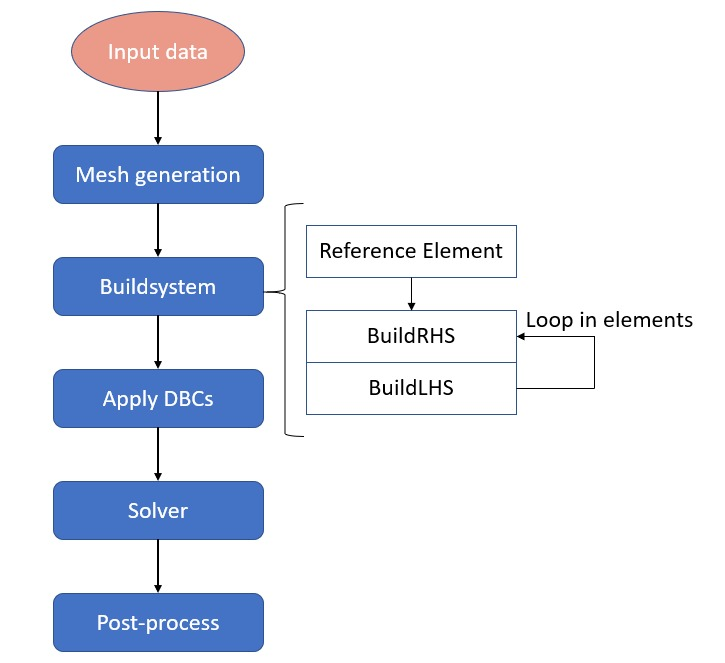
\includegraphics[width=3cm, height= 8cm]{graph.jpeg}
%  
%\end{figure}

\newpage

\subsection{Description of the functions associated to the code}

\vspace{0.3cm}

$\star$ \hspace{0.1cm} \textbf{PREPROCESSING} \\
	
	\begin{myintro}{\textbf{ReferenceElement}}
		\begin{enumerate}
			\item [$\bullet$] \textbf{Inputs}: mesh (\textbf{X} and \textbf{T})
			\item [$\bullet$] \textbf{Outputs}: Reference element data (shape functions, derivatives, locations and weights of the Gauss points) 
			\item [$\bullet$] \textbf{Description}: Creates the reference element that will be used throughout the program. The reference element is defined with respect to the isoparametric variables $\xi$ and $\eta$.
			\item [$\bullet$] \textbf{Uses}: None
			\item [$\bullet$] \textbf{Used by}: Function \textit{BuildSystem}.
			
			\item [$\bullet$] \textbf{Comments}: 
			\begin{enumerate}
				\item [$\star$] Based on the information of the mesh, this function computes and returns the reference element data.
			\end{enumerate}
		\end{enumerate}
	\end{myintro}
	

\vspace{0.5cm}	
\underline{\textbf{Comments on the implementation}}
	
\begin{enumerate}
	\item [$\star$] The input parameters considered on the design of the program are not the same as the ones used on the implementation. We considered that using the type and degree of the elements was a better option when computing the reference element for the problem.
	\item [$\star$] For each type, we define the number of nodes (\textit{nen}) and Gauss points in each element(\textit{ngaus}).
	\item [$\star$] The function \textit{ReferenceElement} calls two new function that respectively calculate the Gauss integration points and weights and the shape functions and their derivatives. They are called \textbf{Quadrature} and \textbf{ShapeFunc}.
	
  	\item [$\star$] The data obtained in this function is stored as a data structure called \textbf{Element}. It will be called throughout the code using the format \textit{Example.value} depending on the information that we seek.
  	
\end{enumerate}




	
	
\end{document}

